\chapter{Concept}
\label{ch:concept}
This chapter presents the theoretical concept of WebArgo as a foundation for the following chapters. The first section defines the terminology used to describe the various actors and entities of WebArgo. Following this, the next section presents WebArgo's architectural design and its key components. The last section of this chapter introduces the underlying theoretical model of WebArgo, which describes the constraints and conditions necessary to achieve potential performance improvement by utilizing the WebArgo platform.

\section{Terminology}
\label{sec:concept:terminology}
This section defines the fundamental terms used to describe all entities and actors of WebArgo. These precise definitions establish all terms used to describe WebArgo's processes in the following chapters of this work.

\subsection{Job}
\label{subsec:concept:job}
A job represents a computational problem or project to be processed or solved by participating volunteers of WebArgo. Jobs are required to be parallelizable, hence a job can be divided into multiple tasks for parallel execution of tasks.

\subsection{Task}
\label{subsec:concept:task}
Each job is divided into multiple tasks and each task ideally has an equal computational workload. Therefore, each task represents a unique, atomic unit of computational workload from its assigned job. Additionally, each task is required to operate independently and therefore requires no communication to other tasks during the execution. These tasks are distributed among the volunteer participants of WebArgo to achieve parallel processing of the entire job.

\subsubsection{Batch}
\label{ssubsec:concept:batch}
A batch is defined to be a subset of tasks, which are all assigned to the same job.

\subsection{Worker}
\label{subsec:concept:worker}
Workers are volunteers who contribute the computational resources of their consumer device to participate in WebArgo and therefore support jobs computed by the WebArgo platform. They receive tasks from the current batch, compute them using their local resources, and transmit the task results to the WebArgo platform.

\subsection{Administrator}
\label{ssubsec:concept:admin}
Administrators manage the WebArgo platform. Therefore, they have the ability to control job execution, monitor overall job progress and monitor the connected workers. Additionally, administrators can develop custom jobs to distribute their project through the WebArgo platform.

\subsection{Backend}
\label{subsec:concept:backend}
The backend is used as the central component to maintain the network. Each client (worker \& administrator) intending to connect to WebArgo must establish a WebSocket connection to the backend. Additionally, the backend is responsible for scheduling and distributing the tasks of a job among all participating workers. Furthermore, the backend is responsible to manage information about all jobs and to persistently store the results of all completed tasks.

\subsection{Frontend}
\label{subsec:concept:frontend}
The frontend enables the connection between workers or administrators and the backend. Furthermore, it represents a interactive \ac{UI} for the connected clients and is responsible to provide the WebAssembly environment for the workers.

\section{Architecture}
\label{sec:concept:architecture}
The WebArgo platform consists of the following three components:
\begin{itemize}
    \item Backend (\autoref{subsec:concept:backend}) handling the distribution of tasks
    \item Frontend (\autoref{subsec:concept:frontend}) providing the interface of the web application for all clients
    \item Database used to persist job and job progress data
\end{itemize}
\autoref{fig:concept:architecture} illustrates the architecture of WebArgo. The web server that hosts the WebArgo platform serves the backend and the frontend on independent ports. Any heterogeneous clients, diverse in hardware and operating system, are able to connect to WebArgo, if they use a web browser that supports WebAssembly, WebSockets and WebWorker. These clients access the platform by connecting to the frontend, which then establishes the WebSocket communication between the client and the backend. Each client (worker \& administrator) always maintains a bidirectional WebSocket connection to the backend. The database is used to persistently store data about jobs and the progress of each job, and is exclusively accessible by the backend.
\begin{figure}[htbp]
    \centering
    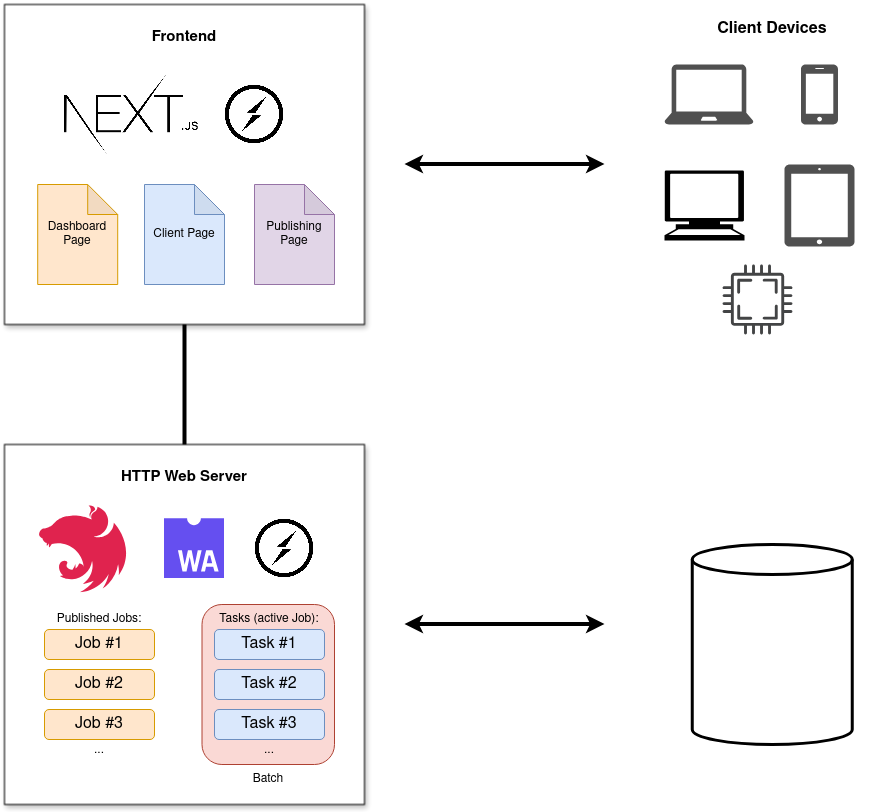
\includegraphics[width=0.95\textwidth]{gfx/figures/WebAssembly-MA.png}
    \caption{Architecture Modell of the Platform}
    \label{fig:concept:architecture}
\end{figure}

\section{Theory}
\label{sec:concept:theory}
This following section presents the mathematical and theoretical background of the developed volunteer computing platform WebArgo. The objective is to identify the constraints that must be satisfied to ensure that the use of WebArgo offers advantages over regular native computing on a single device.

The primary constraint is that the program code, which is distributed across multiple devices, must be capable of parallel execution. This allows all participating devices to each compute a portion of the overall workload simultaneously. In this context, a parallelizable job is characterized by the following properties:
\begin{itemize}
  \item The problem can be divided into multiple tasks
  \item Each task executes the same program code
  \item Each task can receive specific input parameters to process a distinct part of the problem
  \item Each task operates independently, with no need for communication between tasks and no dependencies on other sequentially preceding tasks
\end{itemize}
The total estimated execution time of a job that is divided into \emph{T} tasks which are computing an equal amount of workload and are executed sequentially is denoted as $t_{Seq}$. It is assumed that, on average, each of these tasks requires a computing time of $t_{Native}$ when executed in the native environment. Consequently, the total computation time for the sequential execution of a job on a single device is expressed as:
\begin{equation}
  t_{Seq} = T \cdot t_{Native}
  \label{equ:single}
\end{equation}
When \emph{T} equal tasks are distributed over \emph{W} independent workers, the total computation time is expected to be proportionally reduced, because the workload is being parallelized. This reducing factor \emph{I} represents the amount of iterations needed to distribute all tasks \emph{T} over \emph{W} workers and is described by the fraction of \emph{T} divided by \emph{W}. Since \emph{T} and \emph{W} are part of the natural numbers $\mathbb{N}$ and a single task can not be split into smaller chunks, \emph{I} is also part of the natural numbers $\mathbb{N}$. In order to esure that the result of the fraction is always a natural number the Gaussian ceiling function is applied here. Hence, \emph{I} is given by: 
\begin{equation}
  I = \bigg\lceil\frac{T}{W}\bigg\rceil
  \label{equ:frac}
\end{equation}
Furthermore, when a problem is distributed across \emph{W} workers over a network connection, the networking overhead must be taken into account in the computation of the total execution time $t_{Dist}$. The networking overhead, denoted as $t_{O}$, consists of the time required to send a task to a single worker and the time needed to transmit the result from a single worker to the backend. It is assumed that the WebAssembly binary file, necessary to execute a task, is loaded on all workers in advance and therefore, the additional time required for this initialization process is excluded from the calculation. This networking overhead time can be calculated if the network latency $L$, the network bandwidth $B$ and the file size of the task and result to be transmitted is known. Assuming the average file size of a single task is $F_{T}$ and of a single result is $F_{R}$ the networking overhead can be calculated by:
\begin{alignat}{4}
  t_{O} &= L + \frac{F_{T}}{B} + L + \frac{F_{R}}{B} \nonumber \\
  t_{O} &= 2L + \frac{F_{T} + F_{R}}{B}
  \label{equ:overhead}
\end{alignat}
Additionally, it is assumed that the computation time $t_{Virtual}$ of each task executed in the virtualized environment is equally long across all independent workers \emph{W}. Thus, the total execution time $t_{Dist}$ for a parallelizable job distributed across \emph{W} workers can be expressed as:
\begin{alignat}{4}
  t_{Dist} &= I \cdot (t_{Virtual} + t_{O}) \nonumber \\
  t_{Dist} &= \bigg\lceil\frac{T}{W}\bigg\rceil \cdot (t_{Virtual} + t_{O})
  \label{equ:multiple}
\end{alignat}
The main objective of this approach is to reduce the total computation time of a job by distributing the workload across multiple workers in parallel. This means that the distributed execution time on multiple workers $t_{Dist}$, as described by \eqref{equ:multiple}, must be shorter than the sequential execution time on a single device $t_{Seq}$, as described by \eqref{equ:single}. This leads to the following inequality expression:
\begin{alignat}{4}
  t_{Seq} &> t_{Dist} \nonumber \\
  T \cdot t_{Native} &> \bigg\lceil\frac{T}{W}\bigg\rceil \cdot (t_{Virtual} + t_{O})
  \label{equ:compare}
\end{alignat}
In order to transform this inequality, the term needs to be simplified by substituting the Gaussian bracket. To remove the ceiling function of the Gaussian bracket, the value of \emph{I} can be overestimated by the following term:
\begin{equation}
  I = \bigg\lceil\frac{T}{W}\bigg\rceil \quad < \quad \frac{T}{W} + 1
  \label{equ:frac2}
\end{equation}
This overestimate is used to substitude the value of \emph{I} in function \eqref{equ:multiple} to create following inequality:
\begin{equation}
  T \cdot t_{Native} > \bigg(\frac{T}{W} + 1\bigg) \cdot (t_{Virtual} + t_{O})
  \label{equ:substitution}
\end{equation}
This allows the transformation of the inequality in \eqref{equ:substitution}. The inequality in \eqref{equ:substitution} can be transformed as follows, to estimate a maximum threshold value for $t_{Virtual}$:
\begin{alignat}{4}
  T \cdot t_{Native} &> \bigg(\frac{T}{W} + 1\bigg) \cdot (t_{Virtual} + t_{O}) \nonumber \\
  T \cdot t_{Native} &> \bigg(\frac{T + W}{W}\bigg) \cdot (t_{Virtual} + t_{O}) \nonumber \\
  \frac{T \cdot W \cdot t_{Native}}{T + W} &> t_{Virtual} + t_{O} \nonumber \\
  \frac{T \cdot W \cdot t_{Native}}{T + W} - t_{O} &> t_{Virtual}
  \label{equ:transformation1}
\end{alignat}
In the case of the computation time $t_{Virtual}$ being shorter than this threshold value $\frac{T \cdot W \cdot t_{Native}}{T + W} - t_{O}$ from \eqref{equ:transformation1} with a given amount of tasks $T$ and available workers $W$, the execution time $t_{Dist}$ will be faster than $t_{Seq}$, resulting in a performance gain by distributing the workload $T$ among $W$ workers.
~\\
Furthermore, to estimate a minimum threshold value for the amount of available workers $W$, the inequality in \eqref{equ:substitution} can also be transformed as follows:
\begin{alignat}{4}
  T \cdot t_{Native} &> \bigg(\frac{T}{W} + 1\bigg) \cdot (t_{Virtual} + t_{O}) \nonumber \\
  \frac{T \cdot t_{Native}}{t_{Virtual} + t_{O}} &> \frac{T}{W} + 1 \nonumber \\
  \frac{T \cdot t_{Native}}{t_{Virtual} + t_{O}} - 1 &> \frac{T}{W} \nonumber \\
  \frac{T \cdot t_{Native} - t_{Virtual} - t_{O}}{t_{Virtual} + t_{O}} &> \frac{T}{W} \nonumber \\
  W &> \frac{T \cdot (t_{Virtual} + t_{O})}{T \cdot t_{Native} - t_{Virtual} - t_{O}}
  \label{equ:transformation2}
\end{alignat}
The last expression through the transformation in \eqref{equ:transformation2} results in following constraint: Distributing a parallelizable job across multiple workers is only beneficial if the amount of workers $W$ is larger than the estimated threshold value of $\frac{T \cdot (t_{Virtual} + t_{O})}{T \cdot t_{Native} - t_{Virtual} - t_{O}}$ with a given amount of tasks to execute $T$.

Additionally, the expression from \eqref{equ:frac} can be used to determine the optimal amount of workers \emph{W} for a job divided in \emph{T} tasks of equally sized computational workload. The number of iterations \emph{I} reaches its minimum of $1$ if \emph{W} and \emph{T} are equal. This outcome is intuitive, as in this ideal scenario each worker is rersponsible for a single task and therefore all tasks \emph{T} are executed simultaneously. It can be concluded from \eqref{equ:frac} that the amount of workers \emph{W} should ideally be a divisor of \emph{T} to ensure a efficient utilization of all workers. However, in practice, it should be considered to utilize additional backup workers to account for potential failures or disruptions.

\subsection{Theoretical Example Case}
\label{subsec:concept:theroy_example}
To illustrate the performance gain achieved by the volunteer computing platform WebArgo, both expressions $t_{Seq}$ \eqref{equ:single} and $t_{Dist}$ \eqref{equ:multiple} are plotted in \autoref{fig:background:theoryplot}. To calculate these graphs, an average computation time $t_{Native}$ for a single task was assumed to be 34.97 s, based on the measured average run time of the source code in \autoref{app:code:mandelbrot1} on the system specified in \autoref{app:system:mymachine}. This measurement was repeated with a WebAssembly binary, generated with the source code in \autoref{app:code:mandelbrot2}. The average computation time $t_{Virtual}$ of the same task in a browser environment (Mozilla Firefox 132.0 \cite{background:firefox}) on the system specified in \autoref{app:system:mymachine} was measured at 71.17 seconds, being about 2.04 times slower than the native computation time.
\\~\\
This is an unexpected difference in computation duration between native and WebAssembly code execution, since WebAssembly is promised to perform at near-native speed \cite{methodology:wasm, methodology:wasmW3C}. \citeauthor{background:not-so-fast} stated in their work that WebAssembly shows a significantly worse performance compared to native code, with an average performance gap of 45\% (Firefox) to 55\% (Chrome) and peak slowdowns of 2.08x (Firefox) and 2.5x (Chrome) across measured SPEC \acs{CPU} benchmarks \cite{background:not-so-fast}. This matches the unexpected slowdown of 2.04x measured in the previously mentioned experiment of this work. \citeauthor{background:not-so-fast} identified the following performance issues to be the root cause of the experienced performance gap when using WebAssembly \cite{background:not-so-fast}:
\begin{enumerate}
  \item \emph{Increased Register Pressure}
  \item \emph{Extra Branch Instructions}
  \item \emph{Increased Code Size}
\end{enumerate}
~\\
To calculate the networking overhead $t_{O}$ an internet latency $L$ of 32 ms \cite{backend:latency} and a network bandwidth $B$ of 29 Mbps (3.625 MBps) \cite{backend:latency} was assumed. These values represent the \ac{IQI} estimated round trip time within Europe \cite{backend:latency} and the \ac{IQI} estimated download speed in Europe \cite{backend:latency}. In this theoretical scenario a task represents only the input arguments required to execute the WebAssembly module, as described in the source code of \autoref{app:code:mandelbrot2}. These input arguments consists of seven float values, represented as array of strings with a size of $7$. Since this is a comparatively very small file size, the task file size $F_{T}$ is assumed to be $0$. The \acs{PNG} file generated through the execution of the source code in \autoref{app:code:mandelbrot2} has a size of 699.9 KB, representing the result file size $F_{R}$. Using the function in \eqref{equ:overhead} and based on these values the networking overhead $t_{O}$ is estimated to be 0.257 seconds.

Additionally, in the modeling of this theoretical case is an initial offset time considered, which estimates the time needed to initialize the WebAssembly environment for all participating workers of WebArgo. In this process, each worker is required to download all necessary files in advance to be able to execute the workload of a task. Since this setup process occurs in parallel across all workers, is additional offset time matches the time required for the setup of a single worker. This offset value is again calculated using the \ac{IQI} estimated round trip time and download speed in Europe \cite{backend:latency}. The size of the compiled WebAssembly binary file from the source code in \autoref{app:code:mandelbrot2} is 2.7 MB, and the corresponding \emph{wasm\_exec.js} JavaScript file to setup the WebAssembly environment is 16.7 KB, resulting in a total file size of about 2.717 MB. The time required to download both files to a single node can be estimated using the following expression:
\begin{equation}
  DownloadTime = Latency + \frac{Filesize}{Bandwith} 
  \label{equ:offset}
\end{equation}
Since the bandwidth is given in megabytes per second, while the latency is provided in milliseconds, the latency value needs to be converted to seconds. Using the calculation in \eqref{equ:offset}, the additional offset that is required to set up the platform, in this theoretical case, is estimated to be at least 0.782 s.

The amount of all tasks $T$ is set to 15. Using the inequality in \eqref{equ:transformation2} the threshold of workers $W$ is calcualted to be $W > 2.36$, hence at least three available workers are required to achieve a performance improvement in this theoretical case.

Both graphs in \autoref{fig:background:theoryplot} have been calculated based on the previously mentioned values and the inequality terms \eqref{equ:single} and \eqref{equ:multiple} of \autoref{sec:concept:theory}.
\begin{figure}[htbp]
  \myfloatalign
  \subfloat[Variable amount of workers W]{
     \label{fig:background:theoryA}
     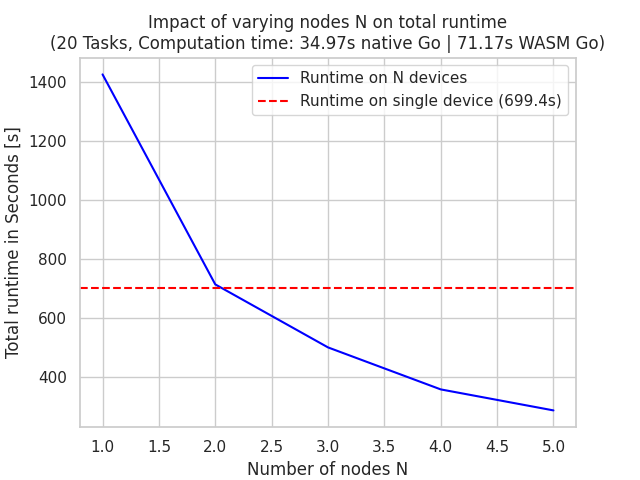
\includegraphics[width=.48\linewidth]{gfx/figures/Theory_A.png}
   } 
   \subfloat[Variable amount of tasks T]{
     \label{fig:background:theoryB}
     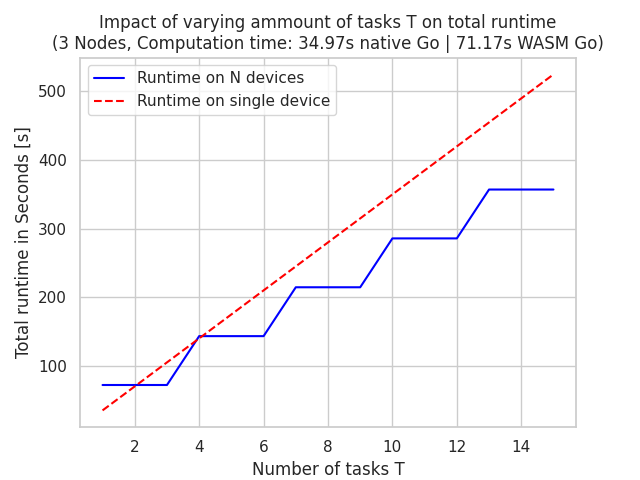
\includegraphics[width=.48\linewidth]{gfx/figures/Theory_B.png}
   }
   \caption{Total Computation Time for an Estimated Example Case}
   \label{fig:background:theoryplot}
\end{figure}
~\\
The graph in \autoref{fig:background:theoryA} represents the total runtime, on the Y-axis in seconds, as a function of the number of workers $W$ in the network, on the X-axis. The red dotted line displays the total execution time $t_{Seq}$ on a single machine, while the blue line illustrates the theoretical total execution time $t_{Dist}$ of WebArgo. The total number of all tasks $T$ is set to 15. This plot validates the expectation, that WebArgo achieves a faster total computation time than a single device, if three or more workers are available. The total runtime $t_{Dist}$ is already by about 35\% faster than $t_{Seq}$ when the workload is distributed to three nodes. 

In summary, this plots illustrates, that the total computation time $t_{Dist}$ is already almost even to the threshold value of $t_{Seq}$ if two workers actively participate in WebArgo and faster if three or more workers participate. This holds true even if the computation time $t_{Virtual}$ of a single task is more than twice as slow in the WebAssembly environment than the computation time $t_{Native}$ on a native system. This proves that the approach of distributing the workload has a performance improvement in this theoretical example, if multiple workers participate in WebArgo. 

However, it needs to be considered, that if only one or two workers participate in WebArgo this approach will always be slower in this example due to the networking overhead, initial offset time and the higher computation time for each individual task.
\\~\\
The other graph in \autoref{fig:background:theoryB} displays the total runtime on the Y-axis in seconds as a function of the number of tasks $T$ on the X-axis. The red dotted line represents again $t_{Seq}$ of a single device and the blue line $t_{Dist}$ of the volunteer computing network. The number of workers $W$ is set to three. This plot demonstrates that WebArgo achieves in this theoretical example a faster total computation time than a single device when the workload $T$ consists of two, three or more than four tasks. The performance gain grows exponentially as the number of tasks increases. Furthermore, it can be concluded that the total computation time $t_{Dist}$ of WebArgo increases in steps, depending on the condition if the number of tasks $T$ and the number of workers $W$ have a common divisor. However, it is crucial to note that the WebArgo platform will have a longer computation time $t_{Dist}$ in every scenario with only one task, as a single task cannot be executed in parallel. Also in the scenario of exactly four tasks $T$ and three workers $W$ the total computation time $t_{Dist}$ is longer than $t_{Seq}$.